\chapter[Resultados Parciais]{Resultados Parciais}



% Dificuldades
% Porcentagem de conclusão
% Conhecimentos adquiridos ( vagrant, bisonc++, flexc++, pesquisa-ação...)
% E-mail com os carinhas
% Cronograma ok

% Objetivo da prova de conceito foi ok
% Contato com orientadores
% Pretende finalizar o gerador. Gerador sintátivo mais completo para a linguagem.

As atividades previstas para a primeira fase do Trabalho de Conclusão de Curso foram executadas com sucesso. Verifica-se que o projeto está com 52,4\%  das suas atividades concluídas. Para essa análise, considerou-se que as atividades descritas nos cronogramas, sendo que utilizou-se um peso de 2 para as atividades da segunda fase do projeto, .

 \begin{figure}[h]
    \centering
    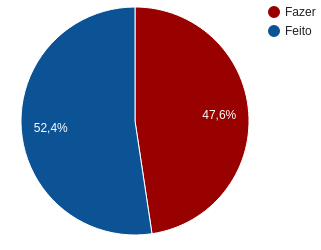
\includegraphics[width=0.5\textwidth]{figuras/pizzadobro.png}
    \caption{ \textit{Status} do Projeto}
    \label{fig:resultados}
 \end{figure}

A Figura  \ref{fig:resultados}